%  DE0.tex
%  Document created by seblovett on seblovett-Ubuntu
%  Date created: Tue 01 Apr 2014 20:11:21 BST
%  <+Last Edited: Fri 04 Apr 2014 14:03:19 BST by hl13g10 on octopus +>

\section{DE0 Implementation}\label{sect:de0}



%\todo[inline]{Use of the slow clock}
A counter was used to slow down the $50MHz$ clock supplied from the board. 
This slowed the processor down to a human usable speed.
The added logic from this is not included in the cost function.


%\todo[inline]{Demo define to allow for easier use during demo.}
To aid the demonstration, a small amount of extra logic is used to show if the opcode is a \texttt{WAIT} instruction. 
This can be turned on or off by used of a \textit{`define} statement declared in the \textit{options.sv} file.
It provides an insight in to the current state of the processor and if it is waiting for an input.

This is accomplished by the code seen in listing \ref{lstleds}.
The logic added by here is not included in the overall cost function and is added to aid the use. 


\lstinputlisting[style=sverilog, firstline=30, lastline=39,caption={Extra LED logic to show when the processor is executing a \texttt{WAIT} instruction.},frame=single,label=lstleds]{../Implementation/cpu.sv}

\subsection{Issues encounterd}

%Program Memory not allowing to be small. 
The ROM was found to be difficult to minimize in size. 
A threshold was found at 512 bits where, if any lower, the module was synthesised into logic elements. 
This could be due to the cost figure for the Altera Synthesis tool to minimize is very different to the cost figure minimized here. 
The use of logic elements would keep the same functionality, but utilises the look up tables in a logic cell. 
The overall cost was still lower using the SRAM, even though a large proportion of the memory is in accessible and remains unused.

\subsection{Synthesis}
%\todo[inline]{Synthesised logic. Put some sexy figures in here}

The extra logic created by the demo definition is shown in figure~\ref{fig:cpudemosynth}.
It consists of two equality checks between the opcode and a constant (the \texttt{WAITn} opcodes).

\begin{figure}
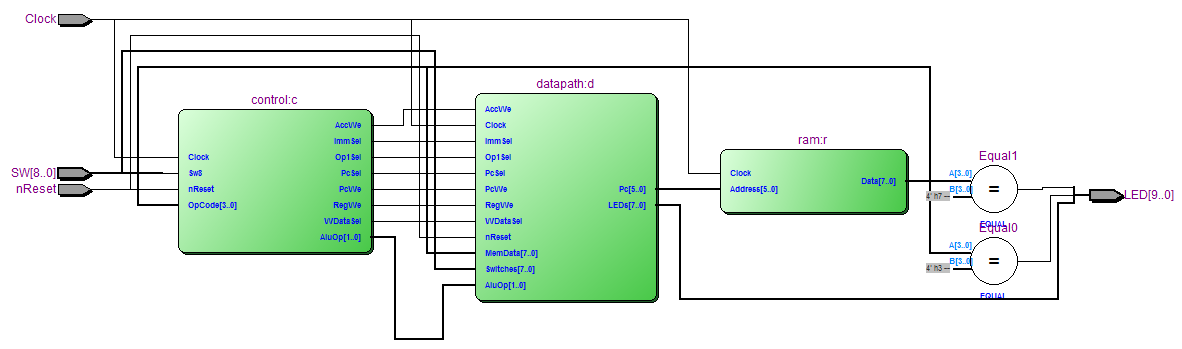
\includegraphics[width=\textwidth]{Figures/cpudemosynth.png}
\caption{Synthesised top level module showing the logic added for the demonstration}
\label{fig:cpudemosynth}
\end{figure}

